\chapter{Contexte Général et État de l'Art}

\section*{Introduction}

Ce premier chapitre établit le contexte général du projet DataWave en présentant l'organisme d'accueil, en analysant la problématique de la gouvernance des données dans les entreprises modernes, en étudiant les solutions existantes sur le marché, et en positionnant DataWave comme une innovation majeure répondant aux limitations identifiées. Nous examinerons les défis actuels de la gouvernance des données, les lacunes des solutions commerciales disponibles, et les avantages compétitifs de notre approche basée sur l'edge computing et l'intelligence artificielle.

\section{Présentation de l'Organisme d'Accueil}

\subsection{Historique et Mission}

% TODO: Remplacer par les informations réelles de votre entreprise d'accueil
[Nom de l'entreprise] est une entreprise [secteur d'activité] fondée en [année] par [fondateurs]. Depuis sa création, l'entreprise s'est positionnée comme un acteur majeur dans le domaine de [domaine d'expertise], avec pour mission de [mission de l'entreprise].

Au fil des années, l'entreprise a connu une croissance significative, passant de [X] employés à sa création à [Y] employés aujourd'hui, avec un chiffre d'affaires de [montant]. Cette évolution témoigne de la pertinence de sa vision et de la qualité de ses services.

\subsection{Domaines d'Activité et Expertise}

L'entreprise opère dans plusieurs domaines d'activité stratégiques :
\begin{itemize}
    \item \textbf{[Domaine 1]} : Description des activités et services
    \item \textbf{[Domaine 2]} : Description des activités et services
    \item \textbf{[Domaine 3]} : Description des activités et services
\end{itemize}

Les technologies maîtrisées incluent [liste des technologies], permettant à l'entreprise de proposer des solutions innovantes à ses clients dans les secteurs [secteurs cibles].

\subsection{Organisation et Structure}

La figure \ref{fig:organigramme} présente l'organigramme de l'entreprise, illustrant sa structure organisationnelle.

\begin{figure}[htpb]
\centering
% TODO: Ajouter l'organigramme de l'entreprise
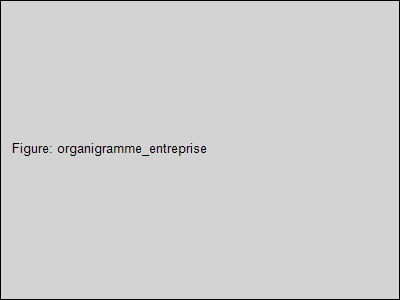
\includegraphics[width=0.8\textwidth]{organigramme_entreprise}
\caption{Organigramme de l'entreprise d'accueil}
\label{fig:organigramme}
\end{figure}

L'entreprise est organisée en [nombre] départements principaux, chacun ayant des responsabilités spécifiques. Notre projet s'inscrit dans le cadre du département [nom du département], qui se concentre sur [responsabilités du département].

\section{Problématique de la Gouvernance des Données}

\subsection{Définition et Enjeux}

La gouvernance des données désigne l'ensemble des processus, politiques, standards, et métriques qui assurent une utilisation efficace et efficiente des données dans une organisation. Elle englobe la gestion de la disponibilité, de l'utilisabilité, de l'intégrité, et de la sécurité des données.

Dans le contexte actuel, la gouvernance des données est devenue critique pour plusieurs raisons :
\begin{itemize}
    \item \textbf{Volume croissant} : Les entreprises génèrent et collectent des volumes de données exponentiels
    \item \textbf{Complexité} : Les données sont dispersées sur de multiples systèmes hétérogènes
    \item \textbf{Conformité} : Les réglementations strictes (GDPR, HIPAA, SOX) imposent des exigences rigoureuses
    \item \textbf{Valeur métier} : Les données sont devenues un actif stratégique pour la compétitivité
\end{itemize}

\subsection{Défis des Entreprises Modernes}

Les entreprises modernes font face à plusieurs défis majeurs en matière de gouvernance des données, comme illustré dans la figure \ref{fig:defis_gouvernance}.

\begin{figure}[htpb]
\centering
% TODO: Créer un diagramme des défis de gouvernance
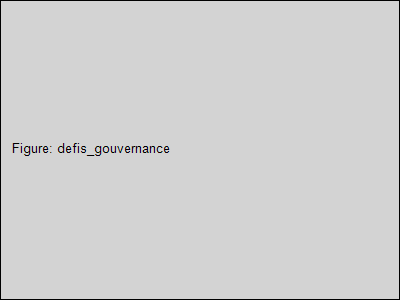
\includegraphics[width=0.9\textwidth]{defis_gouvernance}
\caption{Défis de la gouvernance des données dans l'entreprise moderne}
\label{fig:defis_gouvernance}
\end{figure}

\subsubsection{Silos de Données et Fragmentation}

Les données d'entreprise sont souvent dispersées dans de multiples systèmes isolés (silos), comme illustré dans la figure \ref{fig:silos_donnees}. Cette fragmentation crée plusieurs problèmes :

\begin{itemize}
    \item \textbf{Accès difficile} : Les utilisateurs ne peuvent pas facilement localiser et accéder aux données nécessaires
    \item \textbf{Duplication} : Les mêmes données sont stockées dans plusieurs systèmes, créant des incohérences
    \item \textbf{Qualité variable} : Chaque système maintient ses propres standards de qualité
    \item \textbf{Coûts élevés} : La maintenance de multiples systèmes augmente les coûts opérationnels
\end{itemize}

\begin{figure}[htpb]
\centering
% TODO: Créer un diagramme des silos de données
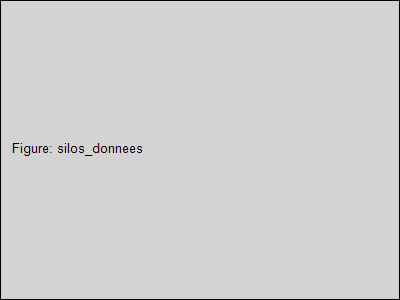
\includegraphics[width=0.85\textwidth]{silos_donnees}
\caption{Silos de données et fragmentation des systèmes}
\label{fig:silos_donnees}
\end{figure}

Le tableau \ref{tab:defis_gouvernance} résume les principaux défis identifiés.

\begin{table}[htpb]
\centering
\caption{Défis de la gouvernance des données}
\label{tab:defis_gouvernance}
\begin{tabular}{|p{0.25\textwidth}|p{0.35\textwidth}|p{0.25\textwidth}|}
\hline
\textbf{Défi} & \textbf{Description} & \textbf{Impact Métier} \\
\hline
Silos de données & Données dispersées sur multiples systèmes isolés & Difficulté d'accès, duplication, incohérences \\
\hline
Conformité réglementaire & Exigences GDPR, HIPAA, SOX, PCI-DSS & Risques légaux, pénalités financières \\
\hline
Qualité des données & Données incomplètes, inexactes, obsolètes & Décisions erronées, perte de confiance \\
\hline
Sécurité & Accès non autorisés, fuites de données & Risques de sécurité, atteinte à la réputation \\
\hline
Traçabilité & Manque de visibilité sur l'origine et les transformations & Difficulté d'audit, non-conformité \\
\hline
\end{tabular}
\end{table}

\subsubsection{Conformité Réglementaire}

Les entreprises doivent se conformer à de multiples frameworks réglementaires, chacun avec ses exigences spécifiques. La figure \ref{fig:frameworks_conformite} présente les principaux frameworks.

\begin{figure}[htpb]
\centering
% TODO: Créer un diagramme des frameworks de conformité
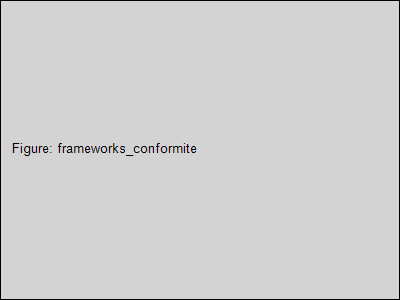
\includegraphics[width=0.9\textwidth]{frameworks_conformite}
\caption{Frameworks de conformité réglementaire (GDPR, HIPAA, SOX, PCI-DSS)}
\label{fig:frameworks_conformite}
\end{figure}

Le tableau \ref{tab:frameworks_reglementaires} détaille ces frameworks.

\begin{table}[htpb]
\centering
\caption{Frameworks de conformité réglementaire}
\label{tab:frameworks_reglementaires}
\begin{tabular}{|p{0.15\textwidth}|p{0.15\textwidth}|p{0.2\textwidth}|p{0.35\textwidth}|}
\hline
\textbf{Framework} & \textbf{Région} & \textbf{Domaine} & \textbf{Exigences Clés} \\
\hline
GDPR & UE & Données personnelles & Consentement, droit à l'oubli, portabilité \\
\hline
HIPAA & USA & Santé & Protection PHI, audit trails, chiffrement \\
\hline
SOX & USA & Finance & Contrôles internes, audit, reporting \\
\hline
PCI-DSS & Global & Paiement & Chiffrement PAN, segmentation réseau \\
\hline
SOC2 & Global & Services cloud & Sécurité, disponibilité, confidentialité \\
\hline
CCPA & Californie & Consommateurs & Transparence, opt-out, non-discrimination \\
\hline
\end{tabular}
\end{table}

\subsection{Besoins Identifiés}

Face à ces défis, les entreprises expriment les besoins suivants :

\begin{enumerate}
    \item \textbf{Support multi-bases de données} : Capacité à gérer tous types de bases de données (relationnelles, NoSQL, cloud warehouses, storage)
    \item \textbf{Classification automatique intelligente} : Utilisation de l'IA/ML pour classifier automatiquement les données sensibles
    \item \textbf{Traçabilité complète} : Data lineage au niveau colonne pour comprendre l'origine et les transformations
    \item \textbf{Conformité automatisée} : Évaluation automatique de la conformité avec génération de rapports
    \item \textbf{Sécurité renforcée} : Contrôle d'accès granulaire avec audit complet
    \item \textbf{Performance et scalabilité} : Capacité à gérer des volumes massifs avec des temps de réponse rapides
\end{enumerate}

\section{Étude des Solutions Existantes}

\subsection{Microsoft Azure Purview}

\subsubsection{Architecture et Fonctionnalités}

Microsoft Azure Purview est une solution de gouvernance des données unifiée qui aide les organisations à gérer et gouverner leurs données on-premises, multi-cloud, et SaaS. La figure \ref{fig:architecture_purview} présente son architecture.

\begin{figure}[htpb]
\centering
% TODO: Créer un diagramme de l'architecture Azure Purview
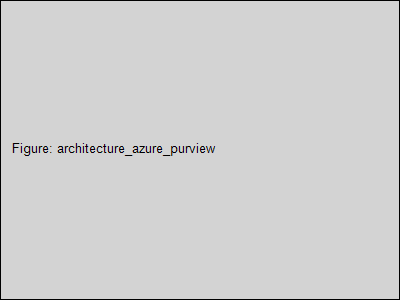
\includegraphics[width=0.9\textwidth]{architecture_azure_purview}
\caption{Architecture de Microsoft Azure Purview}
\label{fig:architecture_purview}
\end{figure}

Les principales fonctionnalités incluent :
\begin{itemize}
    \item Data Map : Cartographie automatisée des données
    \item Data Catalog : Catalogue de données avec recherche
    \item Data Insights : Tableaux de bord et rapports
    \item Data Lineage : Traçabilité des données
\end{itemize}

\subsubsection{Limitations Identifiées}

Malgré ses fonctionnalités, Azure Purview présente plusieurs limitations critiques, illustrées dans la figure \ref{fig:limitations_purview}.

\begin{figure}[htpb]
\centering
% TODO: Créer un diagramme des limitations Azure Purview
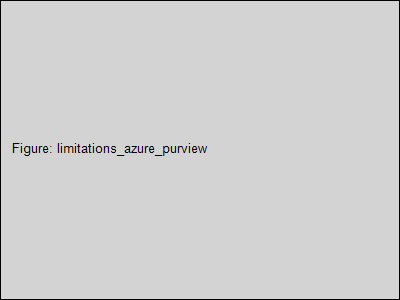
\includegraphics[width=0.85\textwidth]{limitations_azure_purview}
\caption{Limitations et quotas d'Azure Purview}
\label{fig:limitations_purview}
\end{figure}

Le tableau \ref{tab:limitations_purview} détaille ces limitations.

\begin{table}[htpb]
\centering
\caption{Limitations de Microsoft Azure Purview}
\label{tab:limitations_purview}
\begin{tabular}{|p{0.25\textwidth}|p{0.35\textwidth}|p{0.25\textwidth}|}
\hline
\textbf{Catégorie} & \textbf{Limitation} & \textbf{Impact} \\
\hline
Support BD & 3-5 types seulement (SQL Server, Oracle, Teradata) & Couverture limitée \\
\hline
Quotas & 100M assets max, 10 scans concurrents & Scalabilité restreinte \\
\hline
Performance & 250 ops/sec avec 10 capacity units & Throughput limité \\
\hline
Réseau & Pas de support VNet direct & Limitations sécurité \\
\hline
Coûts & Pricing complexe et imprévisible & Budget difficile à contrôler \\
\hline
Vendor lock-in & Dépendance à Azure & Flexibilité réduite \\
\hline
\end{tabular}
\end{table}

\subsection{Databricks Unity Catalog}

\subsubsection{Capacités et Architecture}

Databricks Unity Catalog est une solution de gouvernance unifiée pour les lakehouses. La figure \ref{fig:architecture_databricks} présente son architecture.

\begin{figure}[htpb]
\centering
% TODO: Créer un diagramme de l'architecture Databricks
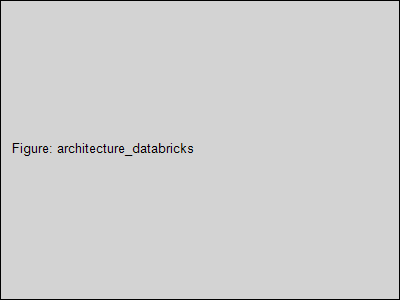
\includegraphics[width=0.9\textwidth]{architecture_databricks}
\caption{Architecture de Databricks Unity Catalog}
\label{fig:architecture_databricks}
\end{figure}

\subsubsection{Contraintes et Limitations}

Le tableau \ref{tab:limitations_databricks} résume les limitations de Databricks Unity Catalog.

\begin{table}[htpb]
\centering
\caption{Limitations de Databricks Unity Catalog}
\label{tab:limitations_databricks}
\begin{tabular}{|p{0.25\textwidth}|p{0.35\textwidth}|p{0.25\textwidth}|}
\hline
\textbf{Aspect} & \textbf{Limitation} & \textbf{Conséquence} \\
\hline
Focus & Optimisé pour processing, pas gouvernance complète & Fonctionnalités limitées \\
\hline
Discovery & Métadonnées basiques seulement & Lineage incomplet \\
\hline
Intégration & Complexe avec systèmes existants & Coûts d'intégration élevés \\
\hline
Coûts & Basés sur compute (imprévisibles) & Budget difficile à planifier \\
\hline
Vendor lock-in & Dépendance Databricks & Flexibilité réduite \\
\hline
Customisation & Limitée & Adaptation difficile \\
\hline
\end{tabular}
\end{table}

\subsection{Autres Solutions}

\subsubsection{Collibra}

Collibra est une solution enterprise complète de gouvernance des données, mais souffre de coûts très élevés et d'une complexité de déploiement importante.

\subsubsection{Alation}

Alation se concentre principalement sur le catalogage avec une intégration limitée et des performances moyennes.

\subsubsection{Informatica}

Informatica propose une suite complète mais complexe, avec des coûts prohibitifs et une courbe d'apprentissage élevée.

\subsection{Analyse Comparative}

Le tableau \ref{tab:comparaison_solutions} présente une comparaison détaillée des solutions existantes.

\begin{table}[htpb]
\centering
\caption{Comparaison des solutions de gouvernance des données}
\label{tab:comparaison_solutions}
\begin{tabular}{|p{0.2\textwidth}|p{0.12\textwidth}|p{0.12\textwidth}|p{0.12\textwidth}|p{0.12\textwidth}|p{0.12\textwidth}|}
\hline
\textbf{Critère} & \textbf{Azure Purview} & \textbf{Databricks} & \textbf{Collibra} & \textbf{Alation} & \textbf{DataWave} \\
\hline
Support BD & 3-5 types & Lakehouse & 10+ types & 8+ types & \textbf{15+ types} \\
\hline
Scalabilité & Limitée & Moyenne & Bonne & Moyenne & \textbf{Illimitée} \\
\hline
IA/ML & Basique & Moyen & Basique & Basique & \textbf{Avancé} \\
\hline
Multi-cloud & Azure only & Limité & Oui & Oui & \textbf{Complet} \\
\hline
Prix & Élevé & Variable & Très élevé & Élevé & \textbf{60-80\% moins} \\
\hline
Performance & Moyenne & Bonne & Moyenne & Moyenne & \textbf{Excellente} \\
\hline
\end{tabular}
\end{table}

\section{Positionnement et Innovation de DataWave}

\subsection{Avantages Compétitifs}

DataWave se positionne comme une solution révolutionnaire qui surpasse les solutions existantes grâce à plusieurs innovations majeures.

\subsubsection{Support Universel de Bases de Données}

DataWave supporte 15+ types de bases de données, contre 3-5 pour les concurrents :
\begin{itemize}
    \item \textbf{Relationnelles} : PostgreSQL, MySQL, Oracle, SQL Server, MariaDB, SQLite
    \item \textbf{NoSQL} : MongoDB, Redis, Elasticsearch
    \item \textbf{Cloud Warehouses} : Snowflake, Redshift, BigQuery, Databricks
    \item \textbf{Storage} : S3, Azure Blob, Google Cloud Storage, REST API
\end{itemize}

\subsubsection{Architecture Edge Computing Révolutionnaire}

L'architecture edge computing de DataWave offre des avantages uniques :
\begin{itemize}
    \item \textbf{Latence réduite} : Traitement au plus près des sources (sub-second)
    \item \textbf{Bande passante optimisée} : Transmission de métadonnées uniquement
    \item \textbf{Scalabilité illimitée} : Scaling horizontal sans limites
    \item \textbf{Conformité locale} : Vérification avant transmission des données
\end{itemize}

\subsubsection{IA/ML Intégré Natif}

DataWave intègre nativement l'intelligence artificielle :
\begin{itemize}
    \item Classification automatique avec 95\%+ de précision
    \item Découverte enrichie par IA
    \item Apprentissage continu
    \item NLP pour recherche sémantique
\end{itemize}

\subsubsection{Multi-Cloud et Hybride}

Support complet de tous les environnements :
\begin{itemize}
    \item AWS, Azure, GCP
    \item On-premises
    \item Hybride avec failover automatique
    \item Pas de vendor lock-in
\end{itemize}

Le tableau \ref{tab:avantages_datawave} résume les avantages compétitifs.

\begin{table}[htpb]
\centering
\caption{Avantages compétitifs de DataWave}
\label{tab:avantages_datawave}
\begin{tabular}{|p{0.3\textwidth}|p{0.3\textwidth}|p{0.3\textwidth}|}
\hline
\textbf{Fonctionnalité} & \textbf{DataWave} & \textbf{Concurrence} \\
\hline
Types de BD supportés & 15+ types & 3-5 types \\
\hline
Architecture & Edge computing & Centralisée \\
\hline
IA/ML & Intégré natif & Basique ou absent \\
\hline
Multi-cloud & Complet (AWS, Azure, GCP) & Limité ou vendor lock-in \\
\hline
Performance & <100ms latency, 1000+ req/sec & Variable, souvent limitée \\
\hline
Coûts & 60-80\% moins cher & Élevés et imprévisibles \\
\hline
\end{tabular}
\end{table}

\subsection{Valeur Ajoutée et Différenciation}

Les figures \ref{fig:positionnement_marche} et \ref{fig:avantages_radar} illustrent le positionnement de DataWave.

\begin{figure}[htpb]
\centering
% TODO: Créer un diagramme de positionnement marché
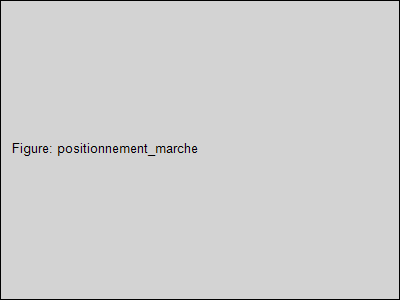
\includegraphics[width=0.85\textwidth]{positionnement_marche}
\caption{Positionnement de DataWave face à la concurrence}
\label{fig:positionnement_marche}
\end{figure}

\begin{figure}[htpb]
\centering
% TODO: Créer un diagramme radar des avantages
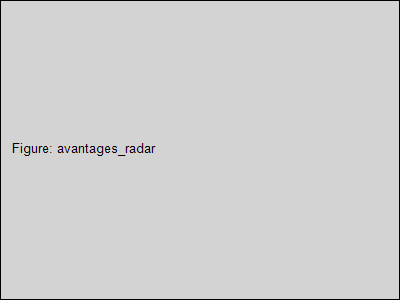
\includegraphics[width=0.8\textwidth]{avantages_radar}
\caption{Avantages compétitifs de DataWave (diagramme radar)}
\label{fig:avantages_radar}
\end{figure}

\subsection{Vision et Roadmap}

\textbf{Court terme (6 mois)} :
\begin{itemize}
    \item Finalisation des 7 modules de gouvernance
    \item Déploiement en production
    \item Validation avec clients pilotes
\end{itemize}

\textbf{Moyen terme (1-2 ans)} :
\begin{itemize}
    \item Extension à d'autres types de BD
    \item Amélioration des modèles IA/ML
    \item Intégration de nouveaux frameworks de conformité
\end{itemize}

\textbf{Long terme (3-5 ans)} :
\begin{itemize}
    \item Plateforme leader du marché
    \item Écosystème de partenaires
    \item Expansion internationale
\end{itemize}

\section*{Conclusion}

Ce chapitre a établi le contexte de notre projet en présentant l'organisme d'accueil et en analysant la problématique de la gouvernance des données. Nous avons identifié les limitations critiques des solutions existantes (Azure Purview, Databricks Unity Catalog) et démontré comment DataWave apporte une innovation majeure grâce à son architecture edge computing, son support universel de bases de données, et son intégration native de l'IA/ML. Le chapitre suivant présentera l'analyse détaillée des besoins et la conception de l'architecture de la plateforme DataWave.
